\documentclass[../main.tex]{subfiles}
 
\begin{document}

\subsection{Macroscopic model}

Macroscopic model describing the intense traffic in one way road as a fluid flow contains three macroscopic variables: the density of cars $\rho$, the average speed $v$, and the flux function $q$, which three can be expressed by the simple convection relation, with the assumption that average speed depends on the density, under condition $t \geqslant 0$ and $x \in \mathbb{R}$:
\begin{equation} \label{eq:1}
    q(\rho) = v(\rho) \, \rho
\end{equation}

N(t) is the number of cars in a particular section $(x_1,x_2)$ of the road, and can be expressed be the following equation, with its derivative on time $t$:
\begin{align} 
    N(t) &= \int_{x_1}^{x_2} \rho(x,t) \, \mathrm{d}x \label{eq:2} \\
    N`(t) &= \frac{d}{dt} \, \int_{x_1}^{x_2} \rho(x,t) \, \mathrm{d}x = \int_{x_1}^{x_2} \rho_t(x,t) \,\mathrm{d}x \label{eq:3}
\end{align}

Because it's assumed that there is no overtaking, "sources", and "sinks", we can derive the conservation law, which summarizes the flux of two borders to get $N`(t)$:
\begin{align}
        N`(t) &= q(\rho(x_1,t)) - q(\rho(x_2,t)) = - \int_{x_1}^{x_2} q(\rho)_x(x,t) \, \mathrm{d}x \label{eq:4}
\end{align}

So we can get \textbf{conservation law for three variables} by eq.\ref{eq:3} minus eq.\ref{eq:4}:
\begin{align}
    \int_{x_1}^{x_2} [\rho_t(x,t) + q(\rho)_x(x,t)] \, \mathrm{d}x &= 0  \label{eq:5} \\
    \begin{split} \label{eq:6}
        \rho_t(x,t) + q(\rho(x,t))_x &= 0 \\
        \rho_t(x,t) + q_x(\rho(x,t)) \, \rho_x &= 0 \\
        \rho_t(x,t) + [v(\rho) \, \rho]_x & =0
    \end{split}
\end{align}

One of the most simplest relationship between $\rho$ and $v$ can be assumed:
\begin{equation}
   v(\rho) = v_m \, \bigg(1 - \frac{\rho}{\rho_m}\bigg) \label{eq:7}
\end{equation}

So that $q$ can be expressed by put $v$ into equation: \ref{eq:1},
\begin{equation}
    q(\rho) &= v_m \, \rho \, \bigg(1-\frac{\rho}{\rho_m}\bigg) \label{eq:8} \\
\end{equation}
    
And we can get $q(\rho)_x$ for eq.\ref{eq:6} to get eq.\ref{eq:10}:
\begin{equation}
    \begin{split} \label{eq:9}
        q(\rho)_x &= q_{\rho}(\rho) \, \rho_x \\
        \frac{\partial \, q(\rho)}{\partial \, x} &= \frac{\partial \, q(\rho)}{\partial \, \rho} \, \frac{\partial \, \rho}{\partial \, x} \\
        &= \left[ v_m \, \rho \, \left(1 - \frac{\rho}{\rho_m}\right)_{\rho} + (v_m \, \rho)_{\rho} \, \left(1 - \frac{\rho}{\rho_m}\right) \right] \, \rho_x \\
        &= \left[ v_m \, \rho \, \left(- \frac{1}{\rho_m}\right) + v_m \, \left(1 - \frac{\rho}{\rho_m}\right) \right] \, \rho_x \\
        &= v_m \, \bigg(1-\frac{2 \rho}{\rho_m}\bigg) \, \rho_x
    \end{split}
\end{equation}

$q(\rho)_x$ can also be expressed:
\begin{align}
    q(\rho)_x = [v(\rho) \, \rho]_x = v \, \rho_x + v_{\rho} \, \rho_x  \rho \label{eq:101}
\end{align}

Above all, we get the partial differential equation problem, of which equation is the only quasi-linear equation for this course, with initial condition assumed:
\begin{align} \label{eq:10}
    \begin{cases}
        \, \rho_t + v_m \, \big(1-\frac{2 \rho}{\rho_m}\big) \, \rho_x = 0 \\
        \, \rho(x,0) = g(x) \\
        \, $t \geqslant 0$ \text{,} $x \in \mathbb{R}$
    \end{cases}
\end{align}

\subsection{The method of characteristics} \label{sec:4.3.2}

To solve the problem, which means to compute the density $\rho$ at a point $(x,t)$ , we follow the idea we already exploited in the linear transport case without external sources:to connect the point $(x,t)$ with a point $(x_0,0)$ on the x-axis, through a curve along which $\rho$ is constant (Fig. \ref{fig:1}).
\\*

\begin{wrapfigure}{\linewidth} \label{fig:1}
\centering
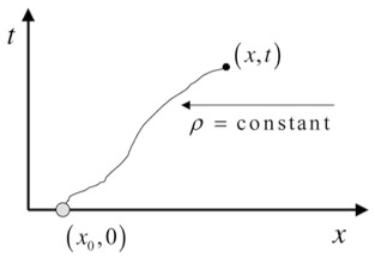
\includegraphics[width = 0.4 \linewidth]{./PDE1-CharacteristicCurve.png}
    \begin{center}
        \text{Figure \ref{fig:1}, Characteristic Curve}
    \end{center}
\end{wrapfigure}
\\*

Clearly, if we manage to find such a curve, that we call characteristic based at $(x_0,0)$, the value of $\rho$ at $(x,t)$ is given by $\rho (x_0, 0) = g (x_0)$. Moreover, if this procedure can be repeated for every point $(x,t)$, $x \in \mathbb{R}$, $t > 0$, then we can compute $\rho$ everywhere in the upper half-plane and the problem is completely solved. This is the \textit{method of characteristics}.

Adopting a slightly different point of view, we can implement the above idea as follows: assume that $x = x (t)$ is the equation of the characteristic based at the point $(x_0,0)$ and that along $x = x (t)$ we always observe the same initial density $g(x_0)$ . In other words, we have:
\begin{align}
    \rho(x(t),t) = g(x_0) \label{eq:11}
\end{align}

for every $t > 0$. If we differentiate the identity from equation \ref{eq:11}, we get:
\begin{align}
    \frac{d}{dt} \rho(x(t),t) = \rho_x(x(t),t) \, x_t(t) + \rho_t(x(t),t) = 0 \label{eq:12}
\end{align}

On the other hand, equation \ref{eq:6} yields the following equation, and the one after substitution of equation \ref{eq:11}: 
\begin{align}
    \rho_t(x(t),t) + q_x(\rho(x(t),t)) \, \rho_x(x(t),t) = 0 \nonumber \\
    \rho_t(x(t),t) + q_x(g(x_0)) \, \rho_x(x(t),t) = 0 \label{eq:13} 
\end{align}

After subtracting equation \ref{eq:12} and equation \ref{eq:13}, we obtain:
\begin{align}
    \rho_x(x(t),t) \, [x_t(t) - q_x(g(x_0))] = 0 \label{eq:14} 
\end{align}

Assuming $\rho_x(x(t),t) \ne 0$, otherwise there is no car on the road, we deduce:
\begin{align}
    x_t(t) = q_x(g(x_0)) \label{eq:15} 
\end{align}

After indefinite integration and $x(0) = x_0$, we get $x(t)$:
\begin{align}
    x(t) = \int x_t(t) \, \mathrm{d}t = q_x(g(x_0)) \, t + x_0 \label{eq:16}
\end{align}

Thus, the characteristics are straight lines with slope $q_x(g (x_0))$. Different values of $x_0$ give, in general, different values of the slope (Fig. 2).
\\*

\begin{wrapfigure}{\linewidth} \label{fig:2}
\centering
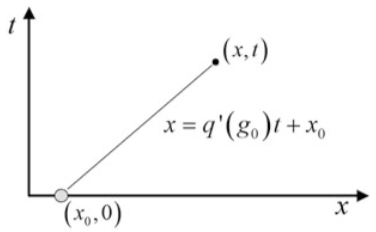
\includegraphics[width = 0.4 \linewidth]{./PDE2-CharacteristicCurve2}
    \begin{center}
        \text{Figure 2, Outcome Characteristic Curve $g_0 = g(x_0)$}
    \end{center}
\end{wrapfigure}
\\*

We can now derive a formula for $\rho(x,t)$, so we move back in time along the characteristic through $(x,t)$ until its base point $(x_0,0)$. Then we can get the following equation with initial condition from equation \ref{eq:10}:
\begin{align}
    \rho(x,t) = \rho(x_0,0) = g(x_0) \label{eq:17}
\end{align}

From equation \ref{eq:16} we have:
\begin{align}
    x_0 = x(t) - q_x(g(x_0)) \, t \label{eq:18}
\end{align}

And we finally get formula for $\rho(x,t)$ after substitute equation \ref{eq:18} in to equation \ref{eq:17}:
\begin{align}
    \rho(x,t) = g(x(t) - q_x(g(x_0))) \label{eq:19}
\end{align}

This equation represents a \textit{travelling wave (or a signal, a disturbance) propagating with speed} $q_x(g (x_0))$ along the positive x-direction.

We emphasize that $q_x(g(x_0))$ is the local wave speed:
\begin{align}
    q_x(g(x_0)) = v_m \, \bigg(1 - \frac{2 \, g(x_0)}{\rho_m} \bigg) \label{eq:20}
\end{align}

And it must not be confused with the traffic velocity. In fact, in general,
\begin{align}
    \frac{d \, q}{d \, \rho} = \frac{d \, (\rho \, v)}{d \, \rho} = v + \rho \, \frac{d \, v}{d \, \rho} \leqslant v \label{eq:21}
\end{align}

The different nature of the two speeds becomes more evident if we observe that the wave speed may be negative as well. This means that, while the traffic advances along the positive x-direction, the disturbance given by the travelling wave may propagate in the opposite direction. Indeed, in our model equation \ref{eq:8}, $d q < 0$ when $\rho > \frac{\rho_m}{2}$ .

Formula \ref{eq:19} seems to be rather satisfactory, since, apparently, it gives the solution of the initial value problem \ref{eq:10} at every point. Actually, a more accurate analysis shows that, even if the initial datum g is smooth, the solution may develop a singularity in finite time (e.g. a jump discontinuity). When this occurs, the method of characteristics does not work anymore and formula \ref{eq:19} is not effective. A typical case is described in Fig. 3: two characteristics based at different points $(x_1, 0)$ and $(x_2, 0)$ intersect at the point (x, t) and the value u (x, t) is not uniquely determined as soon as $g(x_1) ̸= g (x_2)$.
\\*

\begin{wrapfigure}{\linewidth} \label{fig:3}
\centering
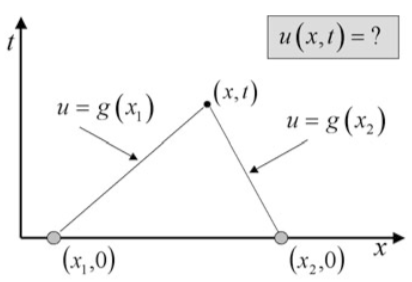
\includegraphics[width = 0.4 \linewidth] {./PDE3-IntersectionCharacteristics}
    \begin{center}
        \text{Figure 3, Intersection of Characteristics}
    \end{center}
\end{wrapfigure}
\\*

In this case we have to weaken the concept of solution and the computation technique. We will come back on these questions later. For the moment, we analyze the method of characteristics in some remarkable cases.

\subsection{The Green Light Problem}

Suppose that bumper-to-bumper traffic is standing at a red light, placed at $x = 0$, while the road ahead is empty. Accordingly, the initial density profile is:
\begin{align} \label{eq:22}
    g(x) = \begin{cases}
               \, \rho_m \quad & \text{for} \, x \leqslant 0 \\
               \, 0 \quad & \text{for} \, x > 0
           \end{cases}
\end{align}

At time $t = 0$, the traffic light turns green and we want to describe the car flow evolution for $t > 0$. At the beginning, only the cars closer to the light start moving while most of them remain standing.

The local wave speed is given by equation \ref{eq:20} after substituting equation \ref{eq:22}:
\begin{align} \label{eq:23}
    q_x(g(x_0)) = \begin{cases}
                      \, - \, v_m \quad & \text{for} \, x_0 \leqslant 0 \\
                      \, v_m \quad & \text{for} \, x_0 > 0
                  \end{cases}
\end{align}

And the characteristics are the straight lines:
\begin{align} \label{eq:24}
    x = \begin{cases}
            \, - \, v_m \, t + x_0 \quad & \text{for} \, x_0 \leqslant 0 \\
            \, v_m \, t + x_0 \quad & \text{for} \, x_0 > 0
        \end{cases}
\end{align}

The lines $x = v_m \, t$ and $x = − \, v_m \, t$ partition the upper half-plane in the three regions $R$, $S$ and $T$, shown in Fig. 4.
\\*

\begin{wrapfigure}{\linewidth} \label{fig:4}
    \centering
    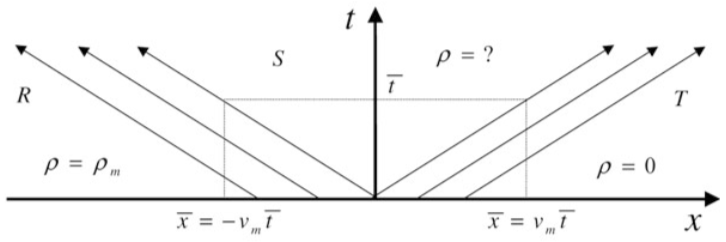
\includegraphics[width = 0.6 \linewidth] {./PDE4-CharacteristicGreenLightProblem}
    \begin{center}
            \text{Figure 4, Characteristic for the Green Light Problem}
    \end{center}
\end{wrapfigure}
\\*

Inside $R$ we have $\rho(x,t) = \rho_m$, while inside $T$ we have $\rho(x,t) = 0$. Consider the points on the horizontal line $t = t_1$. At the points $(x,t_1) \in T$ the density is zero: the traffic has not yet arrived in that area. The front car is located at the point:
\begin{align}
    x_{front} = v_m \, t_1 \label{eq:25}
\end{align}
which moves at the maximum speed, since ahead the road is empty.

The cars placed at the points $(x,t_1) \in R$ are still standing. The first car that starts moving at time $t = t_1$ is at the point:
\begin{align}
    x_{back} = -v_m \, t_1 \label{eq:26}
\end{align}

In particular, it follows that the green light signal propagates back through the traffic at speed $v_m$.

What is the value of the density inside the sector $S$? No characteristic extends into $S$, due to the discontinuity of the initial data at the origin, and the method as it stands does not give any information on the value of $\rho$ inside $S$.

\subsection{Smoothing in the Green Light Problem}

A strategy that may give a reasonable answer is the following:

\begin{enumerate}
  \item Approximate the initial data by a continuous function $g_{\varepsilon}$, which converges to $g$ as $\varepsilon \to 0$ at every point $x$, except 0.
  \item Construct the solution $\rho_{\varepsilon}$ of the $\varepsilon$-problem by the method of characteristics.
  \item Let $\varepsilon \to 0$ and check that the limit of $\rho_{\varepsilon}$ is a solution of the original problem.
\end{enumerate}

Clearly we run the risk of constructing many solutions, each one depending on the way we regularize the initial data, but for the moment we are satisfied if we construct at least one solution.

Let us choose as $g_{\varepsilon}$ the function (Fig. 5):
\begin{align} \label{eq:27}
    g_{\varepsilon} = \begin{cases}
                          \rho_m \quad & x \leqslant 0 \\
                          \rho_m \left(1 - \frac{x}{\varepsilon}\right) \quad & 0 < x < \varepsilon \\
                          0 \quad & x \geqslant \varepsilon
                      \end{cases}
\end{align}
When $\varepsilon \to 0$, $g_\varepsilon(x) \to g(x)$ for every $x \ne 0$.
\\*

\begin{wrapfigure}{\linewidth} \label{fig:5}
\centering
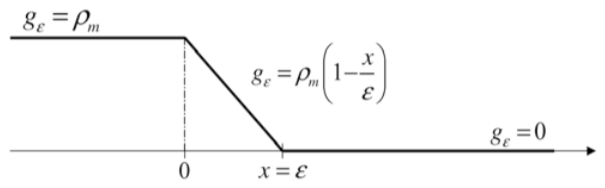
\includegraphics[width=0.7\linewidth]{./PDE5-SmoothingInitialDataGreenLightProblem}
    \begin{center}
        \text{Figure 5, Smoothing of the Initial Data}
    \end{center}
\end{wrapfigure}
\\*

The characteristics for the $\varepsilon$-problem are thus different from equation \ref{eq:24}:
\begin{align} \label{eq:28}
    x &= - \, v_m \, t + x_0 \quad & & \text{if } x_0 < 0 \nonumber \\
    x &= - \, v_m \, \left(1 - 2 \, \frac{x_0}{\varepsilon} \, t + x_0\right) \quad & & \text{if } 0 \leqslant x_0 < \varepsilon \\
    x &= - \, v_m \, t + x_0 \quad & & \text{if } x_0 \geqslant \varepsilon \nonumber
\end{align}

Hence, for $0 \leqslant x_0 < \varepsilon$, the local wave speed (equation \ref{eq:20}) is given by:
\begin{align} \label{eq:29}
    q_x(g(x_0)) = - \, v_m \, \left(1 - 2 \, \frac{x_0}{\varepsilon} \right)
\end{align}

We say that the characteristics in the region $− \, v_m \, t < x < v_m \, t + \varepsilon$ form a rarefaction fan (Fig. 6).
\\*

\begin{wrapfigure}{\linewidth} \label{fig:6}
\centering
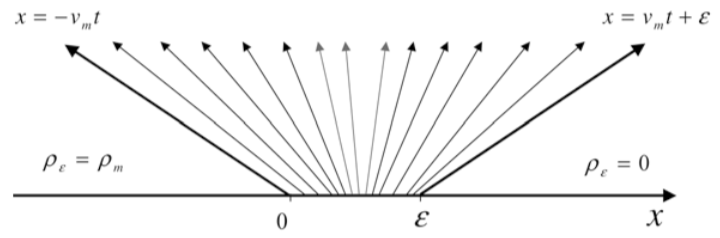
\includegraphics[width=0.7\linewidth]{./PDE6-FanlikeCharacteristics}
    \begin{center}
        \text{Figure 6, Fanlike Characteristics}
    \end{center}
\end{wrapfigure}
\\*

Solving for x0 in the equation of the characteristic (eq. \ref{eq:28}), we get:
\begin{align} \label{eq:30}
    x_0 = \varepsilon \, \frac{x + v_m \, t}{x \, \, t + \varepsilon}
\end{align}

Then we substitute eq. \ref{eq:27} and eq. \ref{eq:30} into eq. \ref{eq:17} to get:
\begin{align} \label{eq:31}
    \rho_{\varepsilon}(x,t) &= g_{\varepsilon}(x_0) \nonumber \\
                            &= \rho_m \, \left(1 - \frac{x_0}{\varepsilon}\right) \nonumber \\
                            &= \rho_m \, \left(1 - \frac{x + v_m \, t}{2 \, v_m \, t + \varepsilon}\right)
\end{align}

Let $\varepsilon \to 0$ in eq. \ref{eq:31}, we obtain:
\begin{align}
    \rho(x,t) = \begin{cases} \label{eq:32}
                \, \rho_m \quad & \text{for } x \leqslant -v_m \, t \\
                \, \frac{\rho_m}{2} \, \left(1 - \frac{x}{v_m \, t} \right) \quad & \text{for } -v_m \, t < x < v_m \, t \\
                \, 0 \quad & \text{for } x \geqslant v_m \, t
                \end{cases}
\end{align}

It is easy to check that $\rho$ is a solution of the equation (4.23) in the regions $R$, $S$, $T$. For fixed $t$, the function $\rho$ decreases linearly from $\rho_m$ to 0, as x varies from $− \, v_m \, t$ to $v_m \, t$. Moreover, $\rho$ is constant on the fan of straight lines:
\begin{align}
    x = h \, t \quad -v_m < h < v_m \label{eq:33}
\end{align}

These type of solutions are called rarefaction or simple waves (centered at the origin). The characteristics and a typical profile are shown in Figs. 7 and Fig. 8.
\\*

\begin{wrapfigure}{\linewidth} \label{fig:7}
\centering
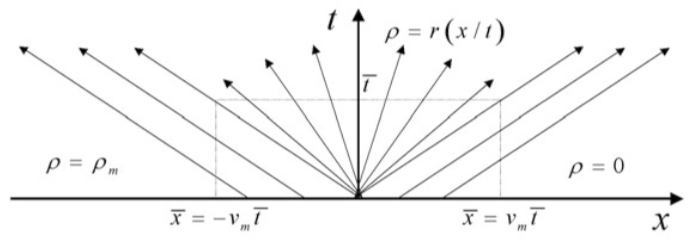
\includegraphics[width=0.7\linewidth]{./PDE7-CharacteristicsRarefactionWave}
    \begin{center}
        \text{Figure 7, Characteristics in a Rarefaction Wave}
    \end{center}
\end{wrapfigure}
\\*

\begin{wrapfigure}{\linewidth} \label{fig:8}
\centering
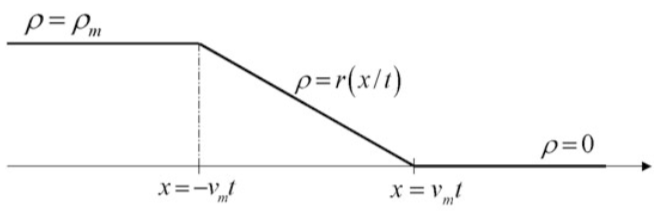
\includegraphics[width=0.7\linewidth]{./PED8-ProfileRarefactionWave}
    \begin{center}
        \text{Figure 8, Profile of a Rarefaction Wave at t}
    \end{center}
\end{wrapfigure}
\\*

\end{document}